\documentclass[12pt]{article}

\usepackage{fullpage}
\usepackage{amsmath,amssymb,amsfonts,amsthm}

\usepackage{ebgaramond}
\usepackage[cmintegrals,cmbraces]{newtxmath}
\usepackage{ebgaramond-maths}

\usepackage{braket}
\DeclareMathOperator{\cas}{cas}
\newcommand{\trans}[1]{\ensuremath{{#1}^\intercal}}

\usepackage{color}

\setlength\parskip{2mm}

\usepackage{graphicx}
\usepackage[hidelinks, colorlinks=true, allcolors=blue]{hyperref}

\usepackage[style=authoryear,backend=bibtex]{biblatex} %backend tells biblatex what you will be using to process the bibliography file
\addbibresource{refs.bib}

\begin{document}
\title{A Survey on Temporal Knowledge Graph Completion: Taxonomy, Progress, and Prospects}
\author{Jiapu Wang et al}
\maketitle


\section{What?}

This is a survey paper about the task of temporal knowledge graph completion. 

\section{Why?}

TKGs or KG in general, ften suffer from incompleteness for three main reasons:
\begin{itemize}
    \item the continuous emergence of new knowledge.
    \item he weakness of the algorithm for extracting structured information from unstructured data.
    \item the lack of information in the source dataset.
\end{itemize}

\section{How?}

The temporal knowledge graph completion task can be divided into two main kinds:
\begin{itemize}
    \item Interpolation: estimates and predicts the missing elements or set of elements through the relevant available
    information.
    \item Extrapolation:  focuses on continuous TKGs and predicts future events, and then classifies all extrapolation methods based on the algorithms
    they utilize.
\end{itemize}

\begin{figure}[h!]
    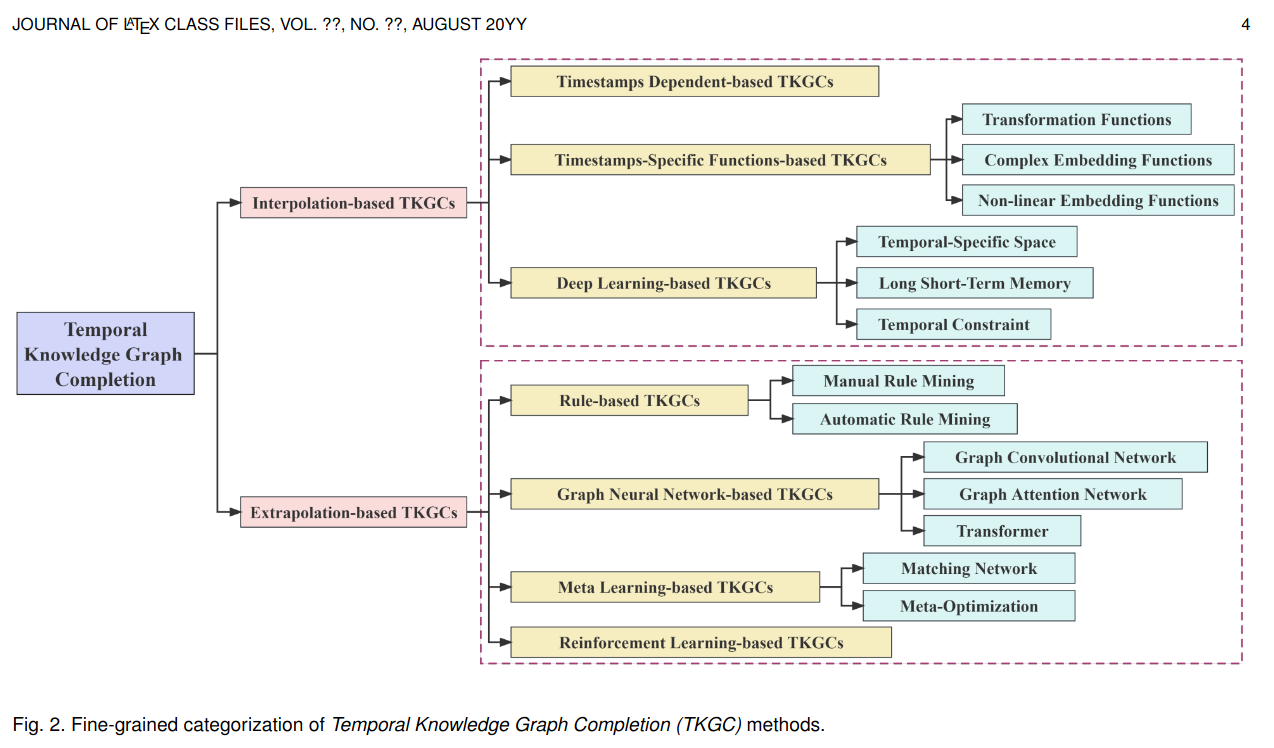
\includegraphics[width=1.1\linewidth]{figures/survey_wang2023_fig01.png}
    \caption{Tổng quan hướng tiếp cận bài toán hoàn thiện đồ thị tri thức động.}
    \label{fig:overview_med_approaches}
\end{figure}

\subsection{Interpolation-based TKGCs}

\subsubsection{Timestamps dependent-based TKGC methods}

These methods typically do not perform operations on timestamps. They just simply
associate the timestamps with the corresponding entity or relation to accomplish
the evolution of entities and relations.

\begin{itemize}
    \item TuckERTNT (\cite{shao2022tucker})
    \item TTransE, ST-TransE
    \item T-SimplE
    \item TKGFrame
    \item TBDRI
\end{itemize}

\subsubsection{Timestamps-specific functions-based TKGC methods}

These methods typically exploit the specific function to learn the embeddings of 
timestamps or the evolution of entities and relations.

There are various useful functions can be used:
\begin{itemize}
    \item Diachronic embedding functions
    \item Gaussian functions 
    \item Transformation functions 
\end{itemize}

Transformation functions: encoding timestamps via one/ or some transformation functions
\begin{itemize}
    \item TransE-ILP (\cite{jiang-etal-2016-towards}) utilize the time-aware embedding model and Integer Linear Programming (ILP) to encode temporal order information and temporal consistency information.
    \item HTTR utilize Householder transformation
    \item BoxTE -> model-agnostic based on BoxTE
    \item SPLIME
    \item TARGCN
    \item TASTER
    \item Time-LowFER
    \item DE-SimplE, DE-DistMult
    \item DEGAT
\end{itemize}

Complex functions: using complex spaces or special coordinate system to capture
various relational patterns.
\begin{itemize}
    \item ChronoR (an extended version of RotatE)
    \item TComplEx and TNTComplEx 
    \item TeRo 
    \item TGeomE (using hypercomplex space, i.e., quaternion)
    \item TeLM (based on TGeomE)
    \item RotateQVS (quaternion space)
    \item ST-NewDE (Dihedron algebra)
    \item BiQCap
    \item HA-TKGE
    \item STKE (spherical coordinate system)
    \item HTKE
\end{itemize}

Non-linear embedding functions: tilize non-linear functions, such as Gaussian and
non-Euclidean functions, to embed TKGs.
\begin{itemize}
    \item DyERNIE, HERCULES
    \item ATiSE
    \item TKGC-AGP
\end{itemize}

\subsubsection{Deep learning-based TKGC methods}

Timestamps-specific space 
\begin{itemize}
    \item HyTE, HTKE, TRHyTE, BTHyTE
    \item ToKEi
    \item SANe
    \item QDN
\end{itemize}

Long short-term memory
\begin{itemize}
    \item TA-TransE, TA-DistMult
    \item TDG2E
    \item TRHyTE
    \item CTRIEJ
    \item TeCre
\end{itemize}

Temporal constraint
\begin{itemize}
    \item Kgedl
    \item T-GAP
    \item TempCaps
    \item RoAN
    \item TAL-TKGC
\end{itemize}

\subsection{Extrapolation-based TKGCs}

\subsubsection{Rule-based TKGC methods}

\begin{itemize}
    \item ALRE-IR
    \item TLogic
    \item TILP
    \item TFLEX
\end{itemize}

\subsubsection{Graph neural network-based TKGC methods}

Graph convolutional network
\begin{itemize}
    \item RE-NET
    \item Glean
    \item TeMP
    \item DACHA
    \item RE-GCN
    \item CyGNet
    \item TiRGN
    \item HiSMatch
    \item SPA
    \item TANGO
    \item HGLS
\end{itemize}

Graph attention network
\begin{itemize}
    \item TPmod
    \item EvoKG
    \item DA-Net
    \item TAE
    \item EvoExplore
    \item CRNet
    \item CENET
    \item MP-KD
    \item Know-Evolve
    \item RTFE
    \item CyGNet
    \item xERTE
    \item T-GAP
\end{itemize}

Transformers
\begin{itemize}
    \item HSAE
    \item rGalT
    \item GHT
\end{itemize}

\subsubsection{Meta learning-based TKGC methods}

Matching network 
\begin{itemize}
    \item FTAG
    \item FTMF
    \item TFSC
\end{itemize}

Meta-optimization
\begin{itemize}
    \item MOST
    \item MetaTKG
    \item MetaTKGR
\end{itemize}

\subsubsection{Reinforcement learning-based TKGC methods}

\begin{itemize}
    \item TAgent (\cite{tao2021temporal})
    \item TPath (\cite{bai2021multi})
    \item TITer (\cite{sun2021timetraveler})
    \item CluSTeR (\cite{li2021search})
    \item DREAM (\cite{zheng2023dream})
    \item RLAT (\cite{bai2023rlat})
\end{itemize}

\printbibliography

\end{document}